\documentclass{article}

\usepackage{amsmath}
\usepackage{amssymb}
\usepackage{parskip}
\usepackage{fullpage}
\usepackage{hyperref}
\usepackage{tikz}
\usepackage{float}
\usepackage{xcolor}

\hypersetup{
    colorlinks=true,
    linkcolor=black,
    urlcolor=blue,
    pdftitle={Differentiation},
    pdfpagemode=FullScreen,
}

\title{Differentiation}
\author{Paolo Bettelini}
\date{}

\begin{document}

\maketitle
\tableofcontents
\pagebreak

\section{Definition}

\subsection{Tangent}

\begin{minipage}{0.5\textwidth}
    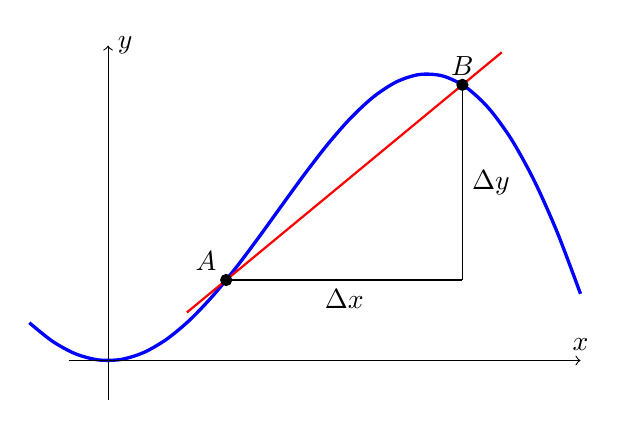
\begin{tikzpicture}[
        scale=2,
        declare function={
            func(\x) = \x*sin(\x r);
            Width=3;
            Height=2;
            Ax=0.75;
            Bx=2.25;
            SlopeMargin=0.25;
            M=(func(Bx) - func(Ax)) / (Bx - Ax);
            Q=func(Ax) - M * Ax;
            slopeFunc(\x)=\x * M + Q;
        }
    ]
        \draw[domain=-0.5:3, smooth, variable=\x, blue, very thick] plot ({\x}, {func(\x)});
        
        \draw[->] (0, -0.25) -- (0, Height) node[right] {\(y\)};
        \draw[->] (-0.25, 0) -- (Width, 0) node[above] {\(x\)};

        \draw[-] (Ax, {func(Ax)}) -- node[below] {\(\Delta x\)} (Bx, {func(Ax)});
        \draw[-] (Bx, {func(Ax)}) -- node[right] {\(\Delta y\)} (Bx, {func(Bx)});
        
        \filldraw [red, thick] ({Ax - SlopeMargin}, {slopeFunc(Ax - SlopeMargin)}) -- ({Bx + SlopeMargin}, {slopeFunc(Bx + SlopeMargin)});
        
        \filldraw [black] (Ax,{func(Ax)}) circle (1pt) node[above left] {\(A\)};
        \filldraw [black] (Bx,{func(Bx)}) circle (1pt) node[above] {\(B\)};
    \end{tikzpicture}
\end{minipage}
\begin{minipage}{0.5\textwidth}
    The mean slope of a function \(f\) between a point \(A\) and \(B\) is given by
    \[
        \frac{\Delta y}{\Delta x} = \frac{f(B)-f(A)}{B-A}
    \]
    As we make \(A\) and \(B\) closer to eachother, \(\Delta x\) decreases.
    As \(\Delta x\) decreases the mean slope is more representative of the rate of change
    of \(f\) in the interval \([A;B]\). \\
\end{minipage}

\begin{minipage}{0.5\textwidth}
    When \(\Delta x\) is infinitely small, we have the precise slope of a given point
    on the function. This slope is represented by the tangent line, which is parallel to the given point.
    \[
        \lim_{\Delta x \to 0} \frac{\Delta x}{\Delta x}
    \]
\end{minipage}
\begin{minipage}{0.5\textwidth}
    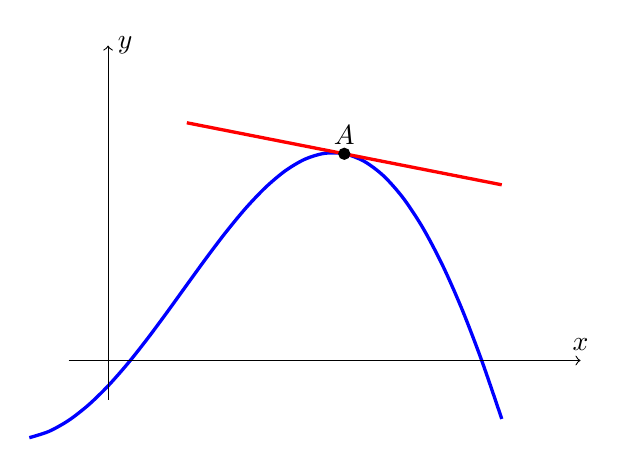
\begin{tikzpicture}[
        scale=2,
        declare function={
            func(\x) = (\x+0.6)*sin((\x+0.6) r)-0.5;
            Width=3;
            Height=2;
            Ax=1.5;
            slope = -0.19697;
        }
    ]
        \draw[domain=-0.5:2.5, smooth, variable=\x, blue, very thick] plot ({\x}, {func(\x)});
        
        \draw[->] (0, -0.25) -- (0, Height) node[right] {\(y\)};
        \draw[->] (-0.25, 0) -- (Width, 0) node[above] {\(x\)};

        \draw[domain=0.5:2.5, smooth, variable=\x, red, very thick] plot ({\x}, {slope * \x + func(Ax) - slope * Ax});
        
        \filldraw [black] (Ax,{func(Ax)}) circle (1pt) node[above] {\(A\)};
    \end{tikzpicture}
\end{minipage}

\subsection{Derivative}

The derivative of a function \(f(x)\) is another function \(f'(x)\) which
represents the rate of change of \(f(x)\). In other words, \(f'(x)\)
represents the slope at each \(x\) of \(f(x)\).

We define \(f'(x)\) by taking the limit of the slope for every \(x\).

\begin{minipage}{0.5\textwidth}
    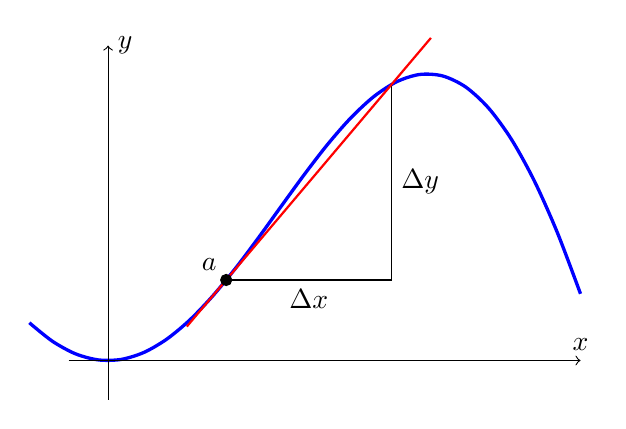
\begin{tikzpicture}[
        scale=2,
        declare function={
            func(\x) = \x*sin(\x r);
            Width=3;
            Height=2;
            Ax=0.75;
            Bx=1.8;
            SlopeMargin=0.25;
            M=(func(Bx) - func(Ax)) / (Bx - Ax);
            Q=func(Ax) - M * Ax;
            slopeFunc(\x)=\x * M + Q;
        }
    ]
        \draw[domain=-0.5:3, smooth, variable=\x, blue, very thick] plot ({\x}, {func(\x)});
        
        \draw[->] (0, -0.25) -- (0, Height) node[right] {\(y\)};
        \draw[->] (-0.25, 0) -- (Width, 0) node[above] {\(x\)};

        \draw[-] (Ax, {func(Ax)}) -- node[below] {\(\Delta x\)} (Bx, {func(Ax)});
        \draw[-] (Bx, {func(Ax)}) -- node[right] {\(\Delta y\)} (Bx, {func(Bx)});
        
        \filldraw [red, thick] ({Ax - SlopeMargin}, {slopeFunc(Ax - SlopeMargin)}) -- ({Bx + SlopeMargin}, {slopeFunc(Bx + SlopeMargin)});

        \filldraw [black] (Ax,{func(Ax)}) circle (1pt) node[above left] {\(a\)};
    \end{tikzpicture}
\end{minipage}
\begin{minipage}{0.5\textwidth}
    We define the derivative as
    \[
        f'(x) = \lim_{\Delta x \to 0} \frac{f(x + \Delta x) - f(x)}{\Delta x}
    \]
    or
    \[
        f'(x) = \lim_{h \to x} \frac{f(h) - f(x)}{x-h}
    \]
\end{minipage}

Using the derivative, the tangent line at \(x=a\) is given by
\[
    y=f'(a)(x-a) + f(a)
\]

\section{Interpretation}

\subsection{Rate of Growth}

Since the derivative \(f'(x)\) represents the rate of change of \(f(x)\),
assuming that \(f(a)\) is defined.
\begin{itemize}
    \item If \(f'(a) > 0\), then \(f(x)\) is increasing at \(x=a\)
    \item If \(f'(a) < 0\), then \(f(x)\) is decreasing at \(x=a\)
    \item If \(f'(a) = 0\), then \(f(x)\) is critical at \(x=a\)
    \item If \(f'(a)\) is not defined, then \(f(x)\) is critical at \(x=a\) (sharp corner)
\end{itemize}
A critical point is when the function is stationary.

A function increases on an interval \(I\) iff
\[
    \forall x_1, x_2 \in I f(x_1) < f(x_2)
\]
and decreases iff
\[
    \forall x_1, x_2 \in I f(x_1) > f(x_2)
\]

\subsection{First Derivative Test}

A critical point \(f'(c)=0\) does not generally imply that \(x=c\) is a minimum or a maximum. 

Let \(f(x)\) be critical at \(x=c\)
\begin{itemize}
    \item If \(f'(x) > 0\) to the left of \(x=c\) and \(f'(x) < 0\) to the right \(x=c\) is a maximum
    \item If \(f'(x) < 0\) to the left of \(x=c\) and \(f'(x) > 0\) to the right \(x=c\) is a minimum
    \item If \(f'(x)\) has the same sign on both sides of \(x=c\) then \(x=c\) is neither.
\end{itemize}
A function may also change sign when it is undefined.

\subsection{Concavity}

\begin{minipage}{0.5\textwidth}
    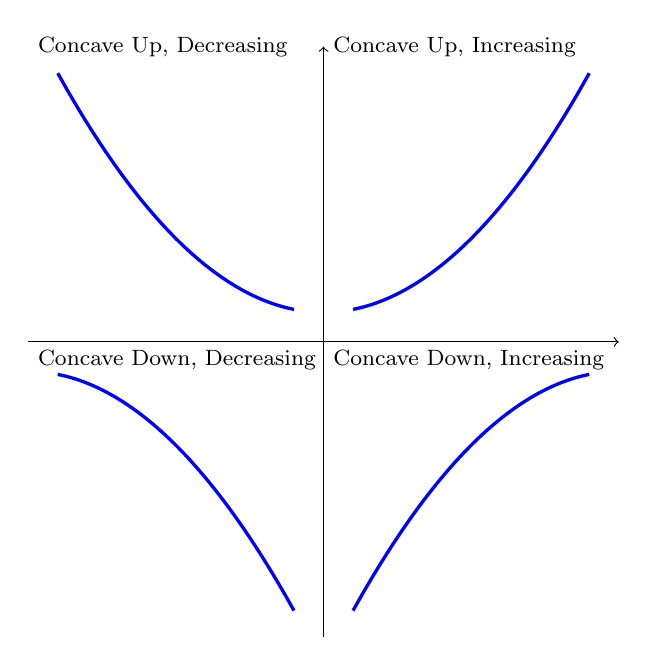
\begin{tikzpicture}[
        scale=1.5,
        declare function={
            func(\x) = \x*\x*0.4;
            Width=5;
            Height=5;
        }
    ]

        \draw[domain=0.25:2.25, smooth, variable=\x, blue, very thick] plot ({\x}, {func(\x - 2.5) + 2.75});
        \draw[domain=2.75:4.75, smooth, variable=\x, blue, very thick] plot ({\x}, {func(\x - 2.5) + 2.75});
        \draw[domain=0.25:2.25, smooth, variable=\x, blue, very thick] plot ({\x}, {-func(\x) + 2.25});
        \draw[domain=2.75:4.75, smooth, variable=\x, blue, very thick] plot ({\x}, {-func(\x - 5) + 2.25});
        
        \node[right] at (0, Height) {\footnotesize Concave Up, Decreasing};
        \node[right] at ({Width / 2}, Height) {\footnotesize Concave Up, Increasing};
        \node[right] at (0, Height / 2 - 0.15) {\footnotesize Concave Down, Decreasing};
        \node[right] at ({Width / 2}, {Height / 2 - 0.15}) {\footnotesize Concave Down, Increasing};
        
        \draw[->] ({Width / 2}, 0) -- ({Width / 2}, Height);
        \draw[->] (0, {Height / 2}) -- (Width, {Height  / 2});
    \end{tikzpicture}
\end{minipage}
\begin{minipage}{0.5\textwidth}
    Functions may present \textbf{concavity}
    \hphantom{ } \\
    \begin{itemize}
        \item \(f(x)\) is \textbf{concave up} on an interval \(I\) iff all of the tangents on \(I\) are below the graph.
        \item \(f(x)\) is \textbf{concave down} on an interval \(I\) iff all of the tangents on \(I\) are above the graph.
    \end{itemize}
    \hphantom{ } \\
    \begin{itemize}
        \item \(f''(x)>0\) for all \(x\) in some interval \(I\) then \(f(x)\) is concave up on \(I\)
        \item \(f''(x)<0\) for all \(x\) in some interval \(I\) then \(f(x)\) is concave down on \(I\)
    \end{itemize}

    This works because when the function is concave up, it increases or decreases more and more. So \(f'(x)\)
    tells us that \(f(x)\) is increasing or decreasing, and \(f''(x)\) tells us the rate at which the increment
    is increasing or the decrease is decrementing. The same goes for when the function is concave down.
\end{minipage}

\pagebreak

An \textbf{inflection point} is a point where the function is continuous and the concavity at that point changes.
Hence, when \(f''(x)\) changes sign we have an inflection point.

\subsection{Second Derivative Test}

Suppose that \(x=c\) is a critical point of \(f(x)\) such that \(f'(x)=0\)
and that \(f''(x)\) is continuous around \(x=c\).
\begin{itemize}
    \item If \(f''(x)<0\) then \(x=c\) is a maximum.
    \item If \(f''(x)>0\) then \(x=c\) is a minumum.
    \item If \(f''(x)=0\) then \(x=c\) could be a maximum, minimum or neither.
\end{itemize}

\section{Absolute Extrema}

When looking for an absolute extrema in a function \(f(x)\), asking when
\(f'(x)=0\) is not enough since the function may not be continuous and have a maxima at a discontinuity point.

\pagebreak

\section{Rules for differentiation}

\[
    \frac{d}{dx}(n)=0
\]

\paragraph{Power Rule}
\[
    \frac{d}{dx}(x^n)=nx^{n-1},\quad n\in\mathbb{R}^*
\]

\[
    \frac{d}{dx}\left(n\cdot f(x)\right)=n\frac{d}{dx}\left(f(x)\right)
\]

\[
    \frac{d}{dx}(f+g)=f'+g'
\]

\paragraph{Product Rule}
\[
    \frac{d}{dx}(f\cdot g)=g'f+gf'
\]

\paragraph{Quotient Rule}
\[
    \frac{d}{dx}\left(\frac{f}{g}\right)=\frac{f'g-fg'}{g^2}
\]

\paragraph{Chain Rule}
\[
    \frac{d}{dx}(f(g(x)))=f'(g(x))\cdot g'(x)
\]

\[
    \frac{d}{dx}(f^g)=f^g\left(\frac{f'g}{f}+g'\ln f\right)
\]

\section{L'Hôpital Rule}

Given the function \(f(x)\) and \(g(x)\) which are differentiable in an open interval \(I\) except
possibly at \(x=c\), if
\[
    \lim_{x\to c} f(x) = \lim_{x\to c} g(x) = 0 \text { or } \pm \infty, \quad g(x\in I) \neq 0
\]
then
\[
    \lim_{x\to c} \frac{f(x)}{g(x)} = \lim_{x\to c} \frac{f'(x)}{g'(x)} 
\]
if such limit exists.

\pagebreak

\section{Intermediate value Theorem}

A function \(f\) continuous on an interval \([a;b]\) will take
every value in the interval \([f(a);f(b)]\).

\section{Bolzano's Theorem}

If \(f(x)\) is continuous on \([a;b]\) and \(f(a)\cdot f(b) <0\) then there is a root.
\[
    f(a)\cdot f(b) <0 \implies \exists c \in [a;b] \mid f(c) = 0
\]

\section{Weierstrass Theorem}

If \(f(x)\) is continuous in \([a;b]\) then the function will have a maxima and a minima.

\section{Rolle's Theorem}
Suppose that \(f(x)\) is continuous on \([a;b]\) and differentiable on \((a;b)\).
\[
    f(a)=f(b) \implies \exists \,c \,|\, f'(c) = 0, \quad
    a < c < b
\]

\section{Mean Value Theorem}

Suppose \(f(x)\) is a function continuous on \([a;b]\) and
differentiable on \((a;b)\), there there exist a number \(c\) such that
\[
    f'(x)=\frac{f(b)-f(a)}{b-a}, \quad a<c<b
\]

\begin{minipage}{0.5\textwidth}
    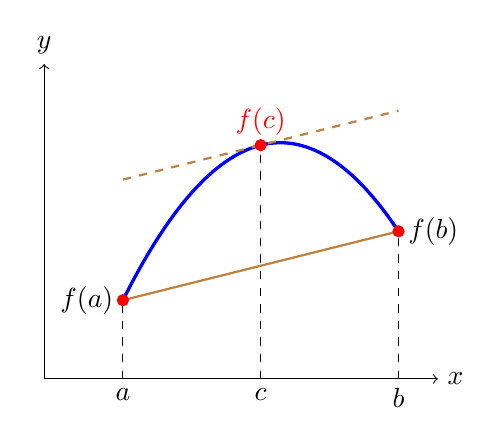
\begin{tikzpicture}[
        declare function={
            func(\x) = - \x * \x * 0.5 + 3 * \x - 1.5;
            a = 1;
            b = 4.5;
            c = 2.75;
            Width=5;
            Height=4;
            m = {(func(b) - func(a)) / (b-a)};
        }
    ]

        \draw[domain=a:b, smooth, variable=\x, blue, very thick] plot ({\x}, {func(\x)});
        \draw[domain=a:b, smooth, variable=\x, brown, thick, dashed] plot ({\x}, {m * \x + 2.28125});
        
        \draw[-, dashed] (a, 0) node[below] {\(a\)} -- (a, {func(a)}) node[left] {\(f(a)\)};
        \draw[-, dashed] (b, 0) node[below] {\(b\)} -- (b, {func(b)}) node[right] {\(f(b)\)};
        \draw[-, dashed] (c, 0) node[below] {\(c\)} -- (c, {func(c)});

        \draw[-, brown, thick] (a, {func(a)}) -- (b, {func(b)});
        
        \filldraw [red] (a,{func(a)}) circle (2pt);
        \filldraw [red] (b,{func(b)}) circle (2pt);
        \filldraw [red] (c,{func(c)}) circle (2pt) node[above] {\(f(c)\)};

        \draw[->] (0, 0) -- (Width, 0) node[right] {\(x\)};
        \draw[->] (0, 0) -- (0, Height) node[above] {\(y\)};
    \end{tikzpicture}
\end{minipage}
\begin{minipage}{0.5\textwidth}
    The mean value on the interval can be represented by the {\color{brown} secant} line.
    What this means is that the interval contains a point whose tangent is equal to the secant.
    \\\\
    Note that if \(f(a) = f(b)\) this is Rolle's theorem.
\end{minipage}

\pagebreak

\section{Chain Rule}

\subsection{Definition}

If \(z\) depends on \(y\), and \(y\) depends on \(x\), then \(z\) also depends on \(x\).
\[
    \frac{dz}{dx}=\frac{dz}{dy}\cdot\frac{dy}{dx}
\]
which is equivalent to
\[
    \frac{d}{dx}(f(g(x)))=f'(g(x))\cdot g'(x)
\]

\subsection{Proof}

Assuming that \(z\) and \(y\) are differentiable in \(x\)

\begin{align*}
    \frac{dz}{dx}
    &= \lim_{\Delta x \to 0} \frac{\Delta z}{\Delta x}
    = \lim_{\Delta x \to 0} \frac{\Delta z}{\Delta y} \cdot \frac{\Delta y}{\Delta x} \\
    &= \left(
        \lim_{\Delta x \to 0} \frac{\Delta z}{\Delta y}
    \right)
    \left(
        \lim_{\Delta x \to 0} \frac{\Delta y}{\Delta x}
    \right) \\
    &= \left(
        \lim_{\Delta x \to 0} \frac{\Delta z}{\Delta y}
    \right)
    \cdot
    \frac{dy}{dx}
\end{align*}

As \(\Delta x \to 0\) also \(\Delta y \to 0\), so we can replace \(\Delta x\) with \(\Delta y\)

\begin{align*}
    \frac{dz}{dx}
    &= \left(
        \lim_{\Delta y \to 0} \frac{\Delta z}{\Delta y}
    \right)
    \cdot
    \frac{dy}{dx} \\
    &= \frac{dz}{dy} \cdot \frac{dy}{dx}
\end{align*}

\section{Differentials}

Given a function \(y = f(x)\) we call \(dy\) and \(dx\) differentials and their relationship is
\[
    dy=f'(x)dx
\]
If we are given just \(f(x)\) then the differentials would be \(df\) and \(dx\)
\[
    df = f'(x)dx
\]

\end{document}